\documentclass[sigconf,review,nonacm]{acmart}

\setcopyright{none}
\settopmatter{printacmref=false,printfolios=true}
\renewcommand\footnotetextcopyrightpermission[1]{}
\pagestyle{plain}

\usepackage{mathtools}
\usepackage{booktabs}
\usepackage{graphicx}
\usepackage{xcolor}
\usepackage{microtype}
\usepackage{enumitem}
\usepackage{listings}
\usepackage{balance}
\emergencystretch=1.5em

\definecolor{contractblue}{HTML}{0072B2}
\definecolor{certgreen}{HTML}{009E73}
\definecolor{warningorange}{HTML}{E69F00}
\definecolor{failurered}{HTML}{D55E00}

\newtheorem{definition}{Definition}
\newtheorem{theorem}{Theorem}
\newtheorem{lemma}{Lemma}
\newtheorem{proposition}{Proposition}

\newcommand{\DecisionSet}{\mathcal{D}}
\newcommand{\FeasiblePairs}{\mathcal{P}}
\newcommand{\Integers}{\mathbb{Z}}
\newcommand{\indicator}{\mathbf{1}}
\newcommand{\figplaceholder}[2]{%
  \fbox{\parbox[c][#2][c]{0.95\linewidth}{\centering\small Image-generation asset pending:\\\texttt{\detokenize{#1}}}}}
\newcommand{\generatedfigure}[3]{%
  \IfFileExists{#1}{\includegraphics[width=#2\linewidth]{#1}}{\figplaceholder{#1}{#3}}}

\title{Bounded Decision Sets: Precision-Hardened Replay for Probabilistic Language Sampling}
\author{Lei Ke}

\begin{document}

\begin{abstract}
Probabilistic language generation can diverge across numerical precisions even when model weights, prompts, and random seeds are fixed. A single changed token alters every later conditional distribution, so a local floating-point discrepancy becomes a trajectory-level failure. Existing replay records either store the whole token trace or certify a narrow boundary condition that can miss support changes. We introduce \emph{bounded decision sets} (BDS), a conservative finite abstraction that enumerates every public sampling decision reachable inside quantized logit intervals. A step is omitted from a replay manifest only when its reachable decision set is a singleton containing the reference token. We prove conditional decision invariance under the declared interval model and show that the procedure terminates in $O(m^2(2\Delta+1)^2)$ time for envelope size $m$ and integer-bin radius $\Delta$. In a frozen FP16-to-BF16 study using Qwen2.5-1.5B-Instruct on one RTX 3060 Laptop GPU, thresholds selected from seed 0 were evaluated without modification on seeds 1 and 2. BDS recovered all 40/40 independent-seed trials across 3,000 token decisions with no observed false-safe step. Its serialized payload was 54.62\% of the matching full trace and 84.70\% of a dual-barrier certificate on the same trials, a 15.30\% relative reduction. These results establish a strong pilot for precision-hardened replay, not a universal floating-point or cross-hardware guarantee. The work contributes a mathematical separation between an explicit perturbation contract and empirical hardware coverage, together with checkpointed code and frozen evidence artifacts.
\end{abstract}

\keywords{probabilistic inference, finite precision, exact replay, language models, discrete contracts, reproducibility}

\maketitle

\section{Introduction}
Stochastic decoding is deceptively stateful. Let $x_t$ be sampled from a next-token distribution conditioned on prefix $x_{<t}$. If two executions select different tokens at time $t$, they no longer evaluate the same distribution at $t+1$. This autoregressive amplification makes ordinary seed synchronization insufficient for replay across numerical environments. It also complicates generative communication methods whose encoder and decoder must make the same public sampling decision from nominally identical probabilities~\cite{wang2025sparsamp,yan2026range}.

The direct engineering response is to record every token. A full trace provides exact reconstruction but costs $\Theta(n\log |V|)$ bits for $n$ steps and vocabulary $V$. Sparse precision replay certificates (SPRCs) instead record only locations where a target environment disagrees with a reference trajectory. Earlier experiments in this repository showed that this delta can be sparse, but they also exposed a harder question: \emph{when can the reference side safely predict that an unobserved target implementation will make the same discrete decision?}

Boundary-radius certificates failed because finite precision changes both the candidate support and the apportioned integer mass. A dual-barrier certificate covered all ten development trials but used 63.02\% of the full trace. A more aggressive local screen used 20.47\% but recovered only 7/10 trials. This is the central reliability--cost tension: a screen is useful only if it is cheap enough to transmit and conservative enough never to omit a decision that can change.

We formulate the problem as finite robust verification. The reference execution publishes an integer envelope rather than a claim about real-valued logits. Each observed logit bin may vary inside a bounded interval. We enumerate feasible top-two supports and all integer-mass contracts reachable inside those supports. Their sampled outputs form a \emph{bounded decision set}. A singleton set certifies local invariance; every other step is recorded. The abstraction is intentionally conservative. It can store an unnecessary token, but under its assumptions it cannot certify two different reachable outputs as one.

This paper makes four contributions:
\begin{itemize}[leftmargin=*]
  \item We define a finite perturbation contract that separates candidate-support uncertainty, mass-apportionment uncertainty, and unknown-tail uncertainty.
  \item We give an exact finite enumeration algorithm and prove conditional soundness, termination, and explicit complexity bounds.
  \item We report a frozen independent-seed pilot: 40/40 exact trials, zero observed false-safe steps, and 54.62\% full-trace payload on 3,000 decisions.
  \item We publish machine-readable result signatures, atomic checkpoints, source-data CSVs, and paired reliability--cost baselines. We also state what the evidence does not establish: cross-hardware validity, distribution preservation, semantic equivalence, or universal numerical error bounds.
\end{itemize}

\begin{figure*}[t]
  \centering
  \generatedfigure{figures/figure_01_architecture.png}{1.0}{4.2cm}
  \Description{Cross-precision replay architecture from FP16 sender through an integer contract and bounded decision set to BF16 replay.}
  \caption{System architecture. The public integer contract converts a precision-sensitive distribution into a finite object. BDS stores only steps whose reachable decision set is not the reference singleton. This non-data illustration is generated from the prompt recorded in \texttt{IMAGEGEN\_PROMPTS.md}.}
  \label{fig:architecture}
\end{figure*}

\section{Background and Problem Statement}
\subsection{Public integer sampling contract}
At step $t$, a model produces logits $\ell_{t,i}$ over tokens $i\in V$. The implementation first selects a public envelope $E_t\subseteq V$ of size $m$, quantizes relative logits with quantum $q>0$,
\begin{equation}
  b_{t,i}=\operatorname{round}\!\left(\frac{\ell_{t,i}-\max_j\ell_{t,j}}{q}\right)\in\Integers,
  \label{eq:bins}
\end{equation}
and chooses the top-$k$ contract support using a public token-identifier tie rule. For support $S_t$, temperature $T$, and integer mass $M=2^B$, define ideal normalized weights
\begin{equation}
  p_i=\frac{\exp(qb_{t,i}/T)}{\sum_{j\in S_t}\exp(qb_{t,j}/T)}.
\end{equation}
The allocator returns integer counts $c_i\ge 0$ with $\sum_i c_i=M$. A public pseudorandom integer $u_t\in\{0,\ldots,M-1\}$ selects the unique token whose cumulative count interval contains $u_t$.

The integer allocator is not distribution-free. For largest-remainder apportionment over $k$ tokens, each coordinate changes by less than $1/M$ after normalization, giving the conservative stepwise bound
\begin{equation}
  \operatorname{TV}(p,c/M)<\frac{2(k-1)}{M}.
  \label{eq:tv}
\end{equation}
For $k=2$ and $B=16$, Eq.~\eqref{eq:tv} is below $3.052\times10^{-5}$. This term excludes top-$k$ truncation and logit quantization; therefore it is neither a zero-KL nor a native-distribution claim.

\subsection{Threat and trust model}
We study reproducible discrete decisions, not concealment against a detector. The sender and receiver share the model identity, tokenizer, prompt, generation parameters, public random context, and integer-contract implementation. Their numerical environments may differ. An adversarial or accidental perturbation is represented only by the declared integer-bin intervals. The replay manifest is authenticated by a surrounding protocol but confidentiality is outside the present experiment.

The target objective is exact token-ID replay. Public surface-text retokenization, model updates, arbitrary kernel changes, and active text modification are outside scope. A certificate may be target-specific. The full trace remains the target-independent upper-cost baseline.

\section{Why Narrow Certificates Fail}
Suppose the reference contract selects token $y_t$. A scalar distance from $u_t$ to the selected cumulative boundary certifies a decision only if candidate support and all earlier integer counts stay fixed. Cross-precision evaluation violates both assumptions. In the R056 development bundle, 12 of 13 observed decision flips were support flips and one was a same-support integer-mass flip (Fig.~\ref{fig:failure}). A scalar boundary radius therefore addresses the least stable representation of the problem.

The failure can be written as a noncommutativity. Let $Q$ quantize logits, $K$ select support, $A$ apportion integer mass, and $F$ sample at public point $u$. In general,
\begin{equation}
F(A(K(Q(\ell))),u)\ne F(A(K(Q(\ell+\varepsilon))),u),
\end{equation}
even when every coordinate of $Q(\ell+\varepsilon)$ is close to $Q(\ell)$. A useful certificate must bound the composite discrete map $F\circ A\circ K$, not an intermediate cumulative boundary alone.

\begin{figure}[t]
  \centering
  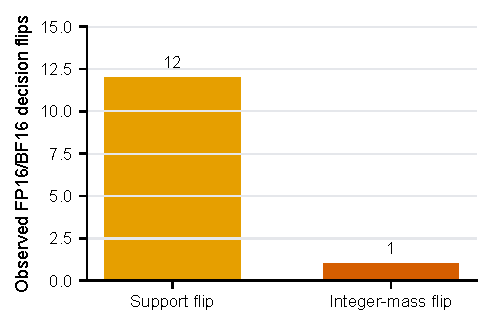
\includegraphics[width=\linewidth]{figures/figure_05_failure_anatomy.pdf}
  \Description{Bar chart showing twelve support flips and one integer-mass flip.}
  \caption{Observed failure anatomy in the frozen R056 development bundle. Support changes dominate but do not eliminate same-support mass changes, motivating joint enumeration.}
  \label{fig:failure}
\end{figure}

\subsection{Research stages as falsification tests}
The sequence R054--R059 was designed to reject weak explanations rather than accumulate favorable configurations. R054 asked whether a conformal radius around the reference cumulative boundary was enough. At its primary radius, it recovered 28/30 development trials, produced two false-safe corrections, and serialized to 115.20\% of the full trace. This simultaneously failed reliability and compression, so neither the split nor the radius was retroactively changed.

R055 then recorded paired FP16/BF16 supports and integer masses at every shared-prefix step. The resulting decomposition identified 12 support flips and one same-support mass flip in the ten-trial held-out development subset. R056 encoded those two mechanisms as separate barriers. It recovered 10/10 trials with no false-safe flip, but 354 of 749 positions required certificates and the 1,416-byte payload was 63.02\% of the 2,247-byte full trace. Under the preregistered efficiency criterion this was a \texttt{no\_go}, despite perfect observed recovery.

R057 tested whether only the nearest support challenger and observed mass-sensitive steps were necessary. Its 460-byte payload was 20.47\% of the full trace, but four of 13 actual flips were omitted and only 7/10 trials were exact. This rejected the hypothesis that one counterfactual challenger captures the support geometry. The omitted cases included a rank-zero reference choice and coupled support/mass movement.

R058 replaced the local challenger with the complete finite set of feasible pairs and bin assignments. On the development subset it recovered 10/10 trials with no false-safe step and used 1,252 bytes, or 55.72\% of the full trace. Because this passed the frozen development gate, and only then, R059 collected untouched seed-1/2 traces. The confirmation did not reuse seed-0 byte totals: it recomputed both BDS and R056 on the same new trajectories.

This progression matters for interpretation. The final method was not selected from an unreported grid of successful variants. Each rejected mechanism left a signed negative artifact and a constraint on the next hypothesis. The result is still exploratory at the field level, but its internal design makes the 40-trial confirmation more informative than an equally sized post-hoc sweep.

\section{Bounded Decision Sets}
\subsection{Interval abstraction}
For each envelope token $i$, the published reference bin $b_i$ induces
\begin{equation}
  L_i=b_i-\Delta,\qquad U_i=b_i+\Delta,
  \label{eq:intervals}
\end{equation}
where $\Delta\in\Integers_{\ge 0}$ is calibrated without target labels from the confirmation set. With top-two sampling, a pair $(i,j)$ is potentially feasible if both can outrank every other observed token:
\begin{equation}
  \min(U_i,U_j)\ge \max_{r\notin\{i,j\}}L_r.
  \label{eq:feasible}
\end{equation}
Let $\FeasiblePairs_t(\Delta)$ be all pairs satisfying Eq.~\eqref{eq:feasible}. For pair $(i,j)$ and candidate bin values $(z_i,z_j)$ in their intervals, let $F_t(\{i,j\},z_i,z_j)$ denote the token selected after public integer apportionment at step $t$.

\begin{definition}[Bounded decision set]
The bounded decision set is
\begin{equation}
\DecisionSet_t(\Delta)=
\bigcup_{(i,j)\in\FeasiblePairs_t(\Delta)}
\left\{F_t(\{i,j\},z_i,z_j):
\substack{z_i\in[L_i,U_i]\cap\Integers,\\z_j\in[L_j,U_j]\cap\Integers}
\right\},
\label{eq:bds}
\end{equation}
augmented by an unknown-tail symbol whenever an unobserved token can enter the top-two support under the envelope bound.
\end{definition}

A step is \emph{certified} exactly when $\DecisionSet_t(\Delta)=\{y_t\}$. Otherwise the manifest records $(t,y_t)$. Figure~\ref{fig:principle} presents the geometric intuition: interval boxes induce feasible supports, feasible supports induce integer partitions, and the public point maps those partitions to a finite output set.

\begin{figure*}[t]
  \centering
  \generatedfigure{figures/figure_02_math_principle.png}{1.0}{4.2cm}
  \Description{Logit intervals generate feasible top-two pairs and a finite set of decisions at a public random point.}
  \caption{Mathematical principle of BDS. The method certifies the composite public decision rather than separately assuming stable support or stable cumulative mass.}
  \label{fig:principle}
\end{figure*}

\subsection{Soundness in the finite model}
\begin{lemma}[Pair coverage]
If an observed token pair can be top two for some assignment $z_r\in[L_r,U_r]$ to all envelope bins, then it satisfies Eq.~\eqref{eq:feasible}.
\end{lemma}
\begin{proof}
For feasible top-two tokens $i,j$, the lower of their assigned values is at least every competing assigned value. Since $z_i\le U_i$, $z_j\le U_j$, and $z_r\ge L_r$, we have $\min(U_i,U_j)\ge\min(z_i,z_j)\ge\max_{r\notin\{i,j\}}L_r$.
\end{proof}

\begin{theorem}[Conditional decision invariance]
Assume (i) every target envelope bin lies in Eq.~\eqref{eq:intervals}; (ii) the target top-two pair is contained in the observed envelope or the tail test raises an alarm; and (iii) sender and receiver use identical public tie-breaking, apportionment, and random point. If $\DecisionSet_t(\Delta)=\{y_t\}$, then the target public contract selects $y_t$.
\end{theorem}
\begin{proof}
By pair coverage, the target pair is in $\FeasiblePairs_t$. Its two realized integer bins appear in the finite enumeration of Eq.~\eqref{eq:bds}. Identical apportionment and public randomness imply the target output belongs to $\DecisionSet_t(\Delta)$. Since this set is the singleton $\{y_t\}$, the output is $y_t$.
\end{proof}

\begin{proposition}[Conservatism and complexity]
For envelope size $m$, BDS tests $\binom{m}{2}$ pairs and at most $(2\Delta+1)^2$ bin assignments per pair. It terminates in $O(m^2(2\Delta+1)^2)$ time and $O(m+|\DecisionSet_t|)$ working space. Enumerating pairwise assignments that cannot coexist with all other bins may add outputs but cannot remove a reachable output.
\end{proposition}

The last statement is the useful asymmetry: over-approximation costs bytes, while under-approximation costs correctness. BDS is designed to fail toward recording.

\subsection{Monotonicity and calibration semantics}
The perturbation radius is not merely a tunable compression parameter. It defines the set of target states for which the theorem is claimed. This gives a useful monotonic structure.

\begin{theorem}[Radius monotonicity]
For $0\le\Delta_1\le\Delta_2$, assume the same envelope and a tail test whose alarm predicate is monotone in $\Delta$. Then
\begin{equation}
  \DecisionSet_t(\Delta_1)\subseteq\DecisionSet_t(\Delta_2).
\end{equation}
Consequently, increasing $\Delta$ cannot turn an unsafe step into a certified step.
\end{theorem}
\begin{proof}
Every integer assignment admitted by $[b_i-\Delta_1,b_i+\Delta_1]$ is also admitted by the wider interval at $\Delta_2$. Equation~\eqref{eq:feasible} can admit additional pairs as upper bounds increase and competitor lower bounds decrease, but it cannot remove an assignment already enumerated at $\Delta_1$. A monotone tail test can only add the unknown-tail symbol. Thus the reachable output set can only grow.
\end{proof}

This theorem makes the reliability--cost control explicit. A larger radius gives a stronger conditional coverage claim but weakly increases the set of recorded steps. Selecting $\Delta$ after examining confirmation labels would therefore invalidate both the statistical separation and the semantic meaning of the contract. Our protocol freezes $\Delta=1$ on development data before R059.

\subsection{Binary mass geometry}
For a feasible pair $(i,j)$ with bins $(z_i,z_j)$, the ideal probability of $i$ is a logistic function of their difference:
\begin{equation}
  p_i(z_i,z_j)=\frac{1}{1+\exp(q(z_j-z_i)/T)}.
  \label{eq:logistic}
\end{equation}
After apportionment, $i$ receives an integer threshold $c_i(z_i,z_j)$ and is selected exactly when the public point satisfies $u_t<c_i$, up to the public token-order convention. Hence BDS need not approximate an arbitrary continuous simplex. It enumerates a small lattice of bin differences and asks whether every reachable integer threshold places $u_t$ on the same side. Support uncertainty adds a finite collection of such lattices.

The geometry explains why a boundary-only method is insufficient. Even if $u_t$ is far from the reference threshold, another feasible support pair can define a different threshold and token order. Conversely, many different bin assignments can collapse to the same integer count and the same selected token, so enumerating decisions can be substantially cheaper to transmit than recording every uncertain probability.

\subsection{Trajectory theorem and manifest cost}
Let $C\subseteq\{1,\ldots,n\}$ be the set of recorded steps and let the manifest contain reference token $x_t$ for each $t\in C$. Replay evaluates the target contract on its current prefix, but applies a stored token before extending that prefix.

\begin{theorem}[Exact trajectory replay]
Assume the conditional decision-invariance theorem holds at every $t\notin C$, every $t\in C$ stores the correct reference token, and replay begins from the reference prompt state. Then replay produces the complete reference trajectory $x_{1:n}$.
\end{theorem}
\begin{proof}
Proceed by induction. The empty generated prefix matches initially. Suppose replay equals $x_{<t}$. Certificate construction and replay therefore evaluate the target contract on the same prefix. If $t\notin C$, conditional invariance selects $x_t$. If $t\in C$, replay substitutes stored token $x_t$ before extension. In both cases the prefix matches through $t$, completing the induction.
\end{proof}

This theorem separates protocol integrity from empirical sparsity. A complete manifest is exact under its stated identities; the measured question is how large $C$ becomes. With sorted correction locations $t_1<\cdots<t_s$, delta-coded positions $d_r=t_r-t_{r-1}$, vocabulary size $|V|$, and a prefix code of length $L(\cdot)$, an idealized payload obeys
\begin{equation}
  B_{\mathrm{BDS}}\le B_{\mathrm{header}}+
  \sum_{r=1}^{s}\left[L(d_r)+\lceil\log_2|V|\rceil\right].
  \label{eq:manifestcost}
\end{equation}
The full trace requires approximately $n\lceil\log_2|V|\rceil$ bits under the same token-ID convention. Equation~\eqref{eq:manifestcost} shows why certificate density alone is not a byte ratio: location coding, headers, trial identities, and token-ID encoding all matter. Our results therefore compare serialized payloads under matching package boundaries.

\subsection{Unknown-tail discipline}
Finite envelopes create a second soundness boundary. Let $b_m$ be the smallest observed envelope bin and let $L_{(2)}$ be the second-largest lower bound among observed tokens. An unobserved token may enter the top-two set whenever
\begin{equation}
  b_m+\Delta\ge L_{(2)}.
  \label{eq:tail}
\end{equation}
When Eq.~\eqref{eq:tail} holds, the implementation inserts \textsc{unknown-tail} into $\DecisionSet_t$ and therefore records the step. It never guesses an unobserved token identity. R059 raised one such alarm. This is costly but honest: the top-16 envelope is an experimental interface, not a proof that all vocabulary logits remain below a fixed bound.

\subsection{Executable correspondence}
The mathematical objects map directly to immutable records. An envelope record contains ordered token identifiers and integer bins. The pair-feasibility loop implements Eq.~\eqref{eq:feasible}. The inner integer loops call the same deterministic allocator and HMAC-derived public point as replay. A witness records feasible-pair count, feasible-contract count, possible token identifiers, tail status, and the final invariant bit.

Three implementation details prevent silent widening of claims. First, token identifiers break all bin and remainder ties; runtime sort stability is not trusted. Second, the target decision is read only after the witness has been constructed, so target labels cannot alter the certificate. Third, the R059 analyzer imports radii from the signed R058 result rather than accepting new command-line thresholds. The analysis can evaluate coverage after construction, but cannot make an unsafe witness safe by seeing the answer.

Synthetic unit tests cover singleton decisions, multiple reachable decisions, support replacement, same-support mass movement, unknown-tail alarms, and invalid negative radii. Experiment checkpoint tests ensure that a changed configuration signature cannot resume into an existing result file. These tests establish code-path behavior; they do not substitute for a proof that a physical GPU lies inside the interval model.

\section{Protocol and Implementation}
The implementation uses a top-16 reference envelope, top-two contract support, $q=0.5$, $T=1.2$, $B=16$, and HMAC-derived public random points. The development phase calibrates three integer thresholds: bin shift $\Delta=1$, same-support mass radius 1,984 counts, and support gap 1 bin. The BDS analysis reads these values from the frozen R058 artifact; it does not infer them from R059 target labels.

For each reference step, the analyzer stores the number of feasible pairs and integer contracts, the candidate decision set, tail-alarm status, and whether a correction is required. Results are written atomically after every trial. Resume is permitted only when the configuration signature matches; an explicit fresh flag archives the old checkpoint before restarting. This preserves completed GPU work and prevents accidental merging across contracts.

\begin{figure*}[t]
  \centering
  \generatedfigure{figures/figure_03_protocol.png}{1.0}{4.0cm}
  \Description{Seed-zero development is separated by a frozen contract from seed-one and seed-two confirmation.}
  \caption{Frozen evaluation protocol. Seed 0 was used for mechanism development. Thresholds and implementation were then frozen before evaluating seeds 1 and 2.}
  \label{fig:protocol}
\end{figure*}

\section{Experimental Methodology}
\paragraph{Model and hardware.}
Experiments use the local Qwen2.5-1.5B-Instruct checkpoint~\cite{qwen2024}, one NVIDIA RTX 3060 Laptop GPU with 6\,GB memory, and sequential FP16/BF16 model loading. The study addresses precision replay on this stack; it is not a multi-hardware benchmark.

\paragraph{Development and confirmation separation.}
R055--R058 used seed 0 for failure diagnosis and method development. R059 used seeds 1 and 2 across 20 fixed English and Chinese prompts, producing 40 trials and 3,000 token decisions. The frozen implementation commit was \texttt{33d14df}; the R058 and R059 result signatures were \texttt{ac2e945...e069} and \texttt{404459f...a60}. Confirmation data did not change thresholds, prompt membership, or acceptance rules.

\paragraph{Outcomes.}
Primary reliability is the count of trials in which every observed FP16/BF16 decision difference is included in the manifest. A \emph{false-safe} step is an actual difference omitted by the certificate. Primary cost is serialized payload divided by a matching full token trace. We additionally report certificate density, tail alarms, and enumeration count. The preregistered strong-go rule required 40/40 exact confirmation trials and lower payload than R056 on the same trajectories.

\paragraph{Comparators.}
R054 is a scalar conformal boundary radius. R056 combines support and integer-mass barriers. R057 is a nearest-challenger local counterfactual screen. R058 is BDS on development trials, and R059 is the independent-seed confirmation. These stages share a research lineage but not identical sample sizes; the frontier is descriptive rather than a significance test.

\section{Results}
\subsection{Reliability--cost frontier}
Figure~\ref{fig:frontier} shows why the BDS result is not a trivial interpolation. R054 used 115.20\% of a full trace and still missed two of 30 trials. R057 reduced cost to 20.47\% but missed three of ten trials. The conservative R056 recovered 10/10 at 63.02\%. BDS recovered 10/10 development trials at 55.72\%, then recovered 40/40 independent-seed trials at 54.62\%.

\begin{figure}[t]
  \centering
  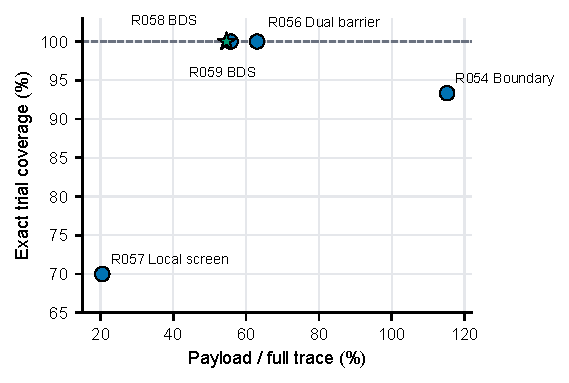
\includegraphics[width=\linewidth]{figures/figure_04_frontier.pdf}
  \Description{Scatter plot of exact trial coverage against payload relative to a full trace for five research stages.}
  \caption{Descriptive reliability--cost frontier across research stages. The star denotes independent-seed confirmation; circles are development evidence.}
  \label{fig:frontier}
\end{figure}

\subsection{Independent-seed confirmation}
Seed 1 recovered 20/20 trials with zero false-safe steps and payload equal to 54.98\% of the full trace. Seed 2 recovered 20/20 at 54.27\%. Pooled, the certificate covered 66 observed FP16/BF16 decision differences across 3,000 decisions, with zero observed false-safe step. One tail alarm correctly forced recording rather than certification.

The pooled manifest contained 4,916 bytes versus 9,000 bytes for the matched full trace, giving 54.6222\%. R056 required 5,804 bytes on the same data; BDS therefore used 84.7002\% of R056, a relative reduction of 15.2998\%. The mean number of enumerated binary integer contracts was 28.584 per token. Certificate locations covered 40.97\% of steps, showing that byte cost and position density are related but not identical.

The per-seed agreement in Fig.~\ref{fig:seeds} is useful because the two seeds induce different trajectories and disagreement locations. Seed 1 contained 1,494 decisions and 38 observed flips; its BDS payload was 2,464 bytes against a 4,482-byte full trace. Seed 2 contained 1,506 decisions and 28 flips; its payload was 2,452 bytes against 4,518 bytes. Their full-trace ratios differed by only 0.70 percentage points even though the observed flip counts differed by ten. The reason is that BDS records uncertainty regions, not only realized target flips. This gap is the price of constructing a source-side certificate without target labels.

Across both seeds, BDS marked 1,229 of 3,000 positions while only 66 positions actually differed. The resulting 18.62-fold payload relative to a target-specific oracle delta is not a contradiction: the oracle reads the target answer, whereas BDS asks which answers are reachable before reading it. R056 was even more conservative on the same data, using 5,804 bytes. The scientific improvement is therefore a reduction in source-side uncertainty cost, not compression toward an unavailable target-conditioned optimum.

\begin{figure}[t]
  \centering
  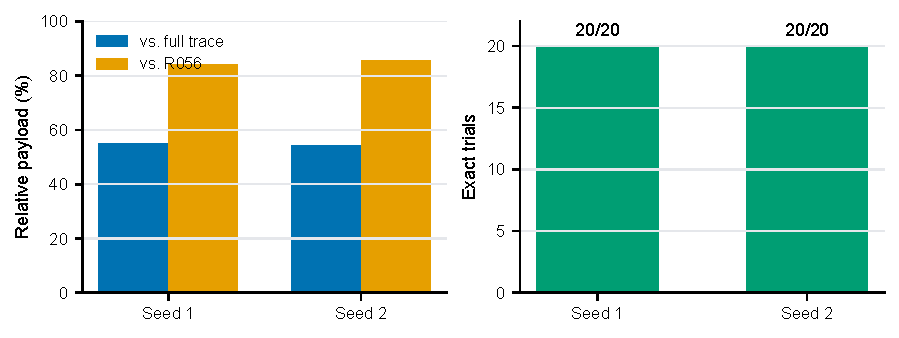
\includegraphics[width=\linewidth]{figures/figure_06_independent_confirmation.pdf}
  \Description{Two-panel chart showing per-seed payload and twenty of twenty exact trials for both independent seeds.}
  \caption{Per-seed confirmation. Both untouched seeds achieved 20/20 exact trial coverage; cost remained stable relative to the full trace and R056.}
  \label{fig:seeds}
\end{figure}

\begin{figure}[t]
  \centering
  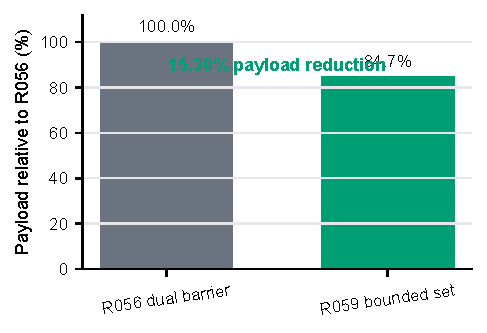
\includegraphics[width=\linewidth]{figures/figure_07_relative_improvement.pdf}
  \Description{Bar chart showing bounded decision set payload at 84.7 percent of the dual-barrier baseline.}
  \caption{Matched payload comparison on R059. BDS reduces serialized payload by 15.30\% relative to the dual-barrier certificate while preserving observed exact coverage.}
  \label{fig:improvement}
\end{figure}

\subsection{Interpretation}
The positive result is narrower than “cross-precision determinism.” BDS certifies decisions only within a calibrated finite box and envelope model. R059 supports seed transfer within one hardware and software stack because thresholds were frozen before seeds 1 and 2 were evaluated. It does not test whether the same box covers a different GPU, CUDA kernel, model revision, or tokenizer. The absence of false-safe steps is therefore empirical coverage evidence layered beneath a conditional theorem, not proof that every future numerical perturbation lies inside the abstraction.

There are two distinct notions of efficiency. Transmission efficiency compares 4,916 BDS bytes with alternative serialized records. Verification efficiency counts 85,752 enumerated contracts over 3,000 token steps, or 28.584 per token. The latter is small because $m=16$ and $\Delta=1$ make the theoretical worst-case $\binom{16}{2}\cdot 3^2=1,080$ contracts per step, while Eq.~\eqref{eq:feasible} rejects most pairs and repeated integer outcomes collapse. We report enumeration count rather than extrapolated wall-clock speed because analysis and GPU inference were not isolated in a controlled timing benchmark.

\section{Security, Distribution, and Semantic Boundaries}
SparSamp established efficient provably secure sampling when encoder and decoder share the required probability contract~\cite{wang2025sparsamp}. Later work showed that finite-precision implementation artifacts can create detectable effects~\cite{cao2026finite}. BDS addresses a complementary implementation layer: reliable agreement on a public discrete sampling decision. It does not itself prove secrecy, indistinguishability, or native-distribution preservation.

Three distribution changes must be reported separately. Top-$k$ truncation removes source mass. Logit quantization changes relative weights. Integer apportionment adds the bounded term in Eq.~\eqref{eq:tv}. Reporting only the retained-support distribution would hide the first two terms. Any future integration with a generative communication system must measure divergence relative to the original model distribution, not only relative to the post-truncation contract.

Likewise, exact token replay is not semantic quality. Qwen was chosen because its instruction-tuned outputs are more coherent than GPT-2 baselines, but the BDS confirmation has no blinded human preference result. Tokenization synchronization such as ReTokSync~\cite{wang2026retoksync} is also orthogonal: the current channel assumes shared token identifiers and tokenizer state.

\section{Related Work}
Provably secure generative sampling couples public model probabilities to a random or message stream. SparSamp reduces sampling cost by exploiting sparse structure~\cite{wang2025sparsamp}; range coding and list-decoding approaches explore alternative capacity and decoding trade-offs~\cite{yan2026range,pang2026list}. Dyadic approximation studies explicit rate--distance trade-offs for language-model outputs~\cite{barlev2026dyadic}. These methods motivate precise probability contracts but generally assume that communicating parties reconstruct compatible discrete distributions.

Numerical nondeterminism in LLM inference arises from reduced precision, kernels, batching, and implementation order~\cite{yuan2025nondeterminism}. Verification systems such as DiFR test outputs despite nondeterminism~\cite{karvonen2025difr}; they do not necessarily reconstruct one stochastic token path. BDS occupies the middle ground between full execution equivalence and outcome-only verification: it certifies a finite public decision abstraction and records the unresolved steps.

\section{Limitations and Research Agenda}
The study has four material limitations. First, all confirmation trials use one physical GPU. A paper-scale claim needs frozen external replay on at least one genuinely independent architecture. Second, $\Delta$ and the mass radius are empirical calibration thresholds rather than analytically derived kernel-error bounds. Third, the prompt set is fixed and small; 40 trials support a pilot contribution but not broad population inference. Fourth, the current result optimizes replay payload, not hidden-channel capacity, output quality, or detector AUC.

The next decisive experiment is a transport test: export only the reference envelope, frozen contract, and code hash to a second GPU stack, then measure coverage without changing thresholds. Failure remains scientifically useful because it identifies which perturbation dimensions escape the finite box. A second line should integrate BDS with a coder on exactly the same integer counts, separating the probability-contract contribution from the coder's capacity. A third line should evaluate public text retokenization and blinded semantic preference as distinct layers.

\section{Threats to Validity}
\paragraph{Construct validity.}
Exact token equality is an unambiguous replay endpoint, but it does not measure semantic quality, indistinguishability, or communication utility. Payload/full-trace ratio is meaningful only under a declared serialization boundary. We use the same trial identities and full-trace encoding for matched comparisons, but comparisons with papers using different headers or message framing would require reserialization.

\paragraph{Internal validity.}
The strongest protection against adaptive analysis is the seed split: R058 froze thresholds and an implementation hash before R059. Nevertheless, seed 0 influenced the mechanism itself, and all stages share the same prompt collection and software lineage. Result signatures detect accidental artifact changes but cannot prove that the implementation realizes the mathematical model. Unit tests on synthetic distributions and exhaustive finite enumeration reduce, rather than eliminate, this risk.

\paragraph{External validity.}
All trials run on one Qwen checkpoint and one RTX 3060 Laptop GPU. Seeds 1 and 2 test stochastic-context transfer, not device transfer. The interval radius may fail to cover another accelerator or kernel even if the finite theorem remains correct. Bilingual prompts broaden surface form but are not a random sample from a defined user population.

\paragraph{Conclusion validity.}
The confirmation result is a census of the configured 40 trials, so we report exact counts rather than a null-hypothesis test. Zero observed false-safe steps does not imply a zero population failure probability. Likewise, the 15.30\% payload reduction is a deterministic difference on the R059 bundle, not an estimate of a universal mean. Paper-scale claims require prompt-cluster uncertainty intervals and independent hardware replication.

\section{Ethics and Reproducibility}
The study uses public model checkpoints, fixed prompts, and locally generated outputs. It does not involve human participants or personal data. The method is presented as a reproducibility and finite-precision audit mechanism. Any integration into a communication system should be evaluated under applicable institutional and legal rules.

The repository includes experiment contracts, checkpoint/resume code, JSON artifacts, SHA-256 material identifiers, source-data CSVs, PDF/PNG figures, and the paper source. The code gate at drafting time was 300 passing tests plus Ruff and a successful Vue/Vite production build. The R059 result is bound to its frozen implementation and result signatures; changing the configuration invalidates resume and requires a new run label.

\section{Conclusion}
Bounded decision sets replace a fragile scalar-boundary intuition with finite verification of the complete public sampling decision. Under a declared integer interval model, singleton decision sets give a simple conditional invariance theorem; non-singletons fail conservatively toward recording. Frozen independent-seed experiments recovered 40/40 tested Qwen FP16-to-BF16 trajectories while reducing matched dual-barrier payload by 15.30\%. This is a credible precision-hardened replay pilot and a concrete mathematical contribution, but its strongest unanswered question is external hardware coverage. The distinction between theorem assumptions and empirical coverage is therefore not a caveat appended to the result; it is the organizing principle of the method.

\balance
\bibliographystyle{ACM-Reference-Format}
\bibliography{references}

\appendix
\section{Finite Enumeration Pseudocode}
\begin{lstlisting}[basicstyle=\ttfamily\scriptsize,frame=single,breaklines=true]
for each token i: [L_i, U_i] <- [b_i-Delta, b_i+Delta]
D <- empty set
for each pair (i,j):
    if min(U_i,U_j) < max_{r not i,j} L_r: continue
    for z_i in [L_i,U_i], z_j in [L_j,U_j]:
        counts <- public_integer_mass(i,j,z_i,z_j)
        D <- D union sample(counts, public_point)
if tail_can_enter_top2(): D <- D union UNKNOWN_TAIL
certify iff D == {reference_token}
\end{lstlisting}

\section{Primary Confirmation Numbers}
The R059 bundle contains 40 trials, 3,000 token decisions, 66 observed decision flips, 1,229 recorded certificate steps, one tail alarm, 85,752 enumerated contracts, 4,916 payload bytes, and 9,000 matching full-trace bytes. Seed-specific full-trace ratios are 54.9755\% and 54.2718\%. All values are read from \nolinkurl{outputs/R059_independent_bounded_decision.json}; the plotting script does not duplicate them as constants.

\end{document}
